\documentclass[a4paper,11pt]{scrartcl}

\usepackage[utf8]{inputenc}
\usepackage[ngerman]{babel}
\usepackage[T1]{fontenc}
\usepackage{amsmath}
\usepackage{graphicx}
\usepackage{tabularx}
\usepackage[a4paper, left=2cm, right=2cm, top=2.8cm, bottom=2.8cm]{geometry}
\usepackage{tikz}   
\usepackage[scaled]{helvet}
\usepackage{tabto} 
\usepackage{fancyhdr}
\usepackage{multirow}

\renewcommand*{\familydefault}{\sfdefault}

\pagestyle{fancy}

\setkomafont{section}{\huge}
\setkomafont{subsection}{\Large}


\lhead{Maximilian Hoffmann}
\chead{Betrieblicher Auftrag \\ \textbf{Kabeltester}}
\rhead{
\includegraphics[width=3cm]{Bilder/BMK_LOGO.png}}

\begin{document}

\section{Blockschaltbild}
	
\begin{center}
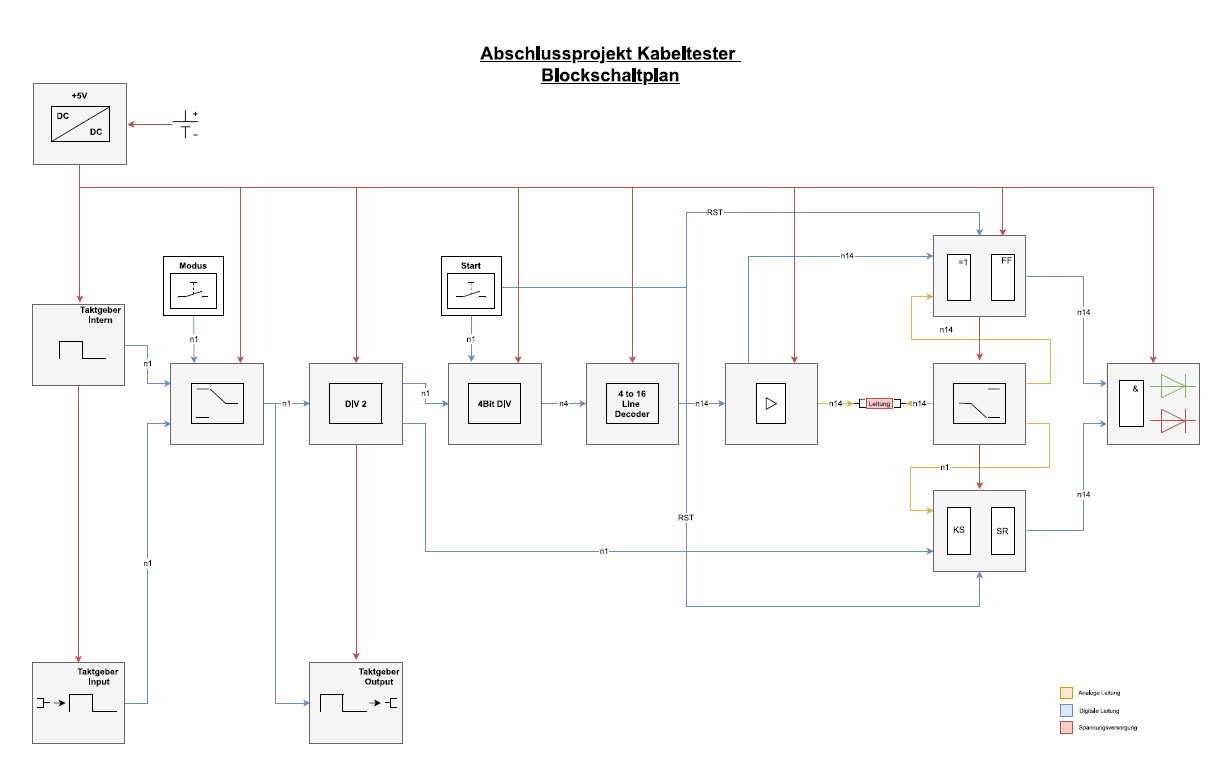
\includegraphics[width=22cm, angle=-90]{Bilder/Blockschaltplan.png}
\end{center}

\newpage

Die Kernfunktion der Messplatine wird in diesem Dokumentationsteil anhand des Blockschaltbildes erklärt. 
\\
\\
Die Versorgung dieser Platine soll durch einen 9V Batterieblock erfolgen. Die Spannung wird dabei durch einen DC/DC - Wandler auf 5V gewandelt.
\\
Ein interner sowie externen Takt kann Wahlweise als Systemtakt verwendet werden. Über einen Taster kann zwischen diesen Taktquellen umgeschaltet werden.
\\
Der Systemtakt wird für das Verwenden mehrerer Messplatinen hintereinander, auf einen Stecker herausgeführt.
\\


\end{document}